\chapter{プロトタイピング}
\label{prototyping}
本章では、手指の変換表現についての探索と、\textit{grasp}が生じる体験として作品を構成するにあたっての取捨選択のプロセスを説明し、最終的な作品における構成の根拠を示す。

\section{プロトタイプの分類}
本研究では、手指の変換表現を通して\textit{grasp}が生じる表現や構成を探索した。
最終的な作品形態に至るまでに、総計60パターンのプロトタイプ制作を行なった。

手指の変換表現の中でも、単に形を考えるだけでなく、どの動きをその形に当てはめるか、そしてどの時間の動きを用いるか等、さまざまな変換方法が考えられる。この段階では先入観によって絞り込むことがないよう、このような探索空間の中で思いつく限り実装し、実際に体験することを通して判断するという姿勢でプロトタイピングをおこなった。以下では、行ったプロトタイピングについて、「形状」、「構造」、「時間操作」の観点から分類する。その上で、これらのプロトタイピングを通してどのような知見を得て、次の探索へつながったのかについての説明を「振り返り」としてこの節の最後に述べる。

\subsection{形状}
形状については、指を1つのユニットとして捉えて、ユニット自体の形状やそれらをどのように関連づけるのかについて検討したもの、そうした枠組みとは無関係に制作したものとの2つに大別できる。
\subsection*{指をユニットと捉えたバリエーション}
指を動きの最小単位として、指ごとに独立したバリエーション、指同士を直列に繋ぎ合わせたバージョン、円形に繋ぎ合わせたバージョンなどを作成した。また、単位である指をどのように表現するかについては、「円形」、「くの字」、「ひょうたん型」などのバリエーションで表現を試みた。
\begin{figure}[H]
  \centering
  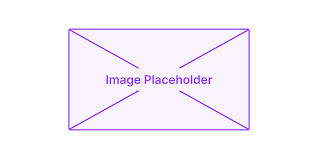
\includegraphics[width=15cm]{img/placeholder.png}
  \caption{ユニットのバリエーション}
  \label{fig:unit_valiation}
\end{figure}

また、これらユニットをいかに繋ぎ合わせて1つの形にするかについても探索を行なった。以下は、同じ「くの字」のユニットについて、「並列に並べたもの」、「片手ずつ直列に繋ぎ、左右の同じ指の高さを結ぶ直線の傾きで回転をかけたもの」、「円形に繋げたもの」の3つのバリエーションである。

\begin{figure}[H]
  \centering
  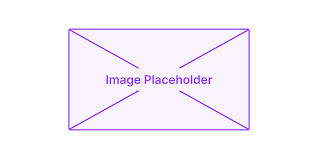
\includegraphics[width=15cm]{img/placeholder.png}
  \caption{繋ぎ方のバリエーション}
  \label{fig:connection_valiation}
\end{figure}

\subsection*{指をユニットとしないバリエーション}
手指の動きを全て包み込む皮膜を「凸包(convex envelope)」のアルゴリズムを用いて実装したり、また指先と付け根の動きだけでなく、指の関節の開き具合を変数として、二等辺三角形の頂角の大きさが変化するバリエーションなどを作成した。

\subsection{マッピング}
マッピングについては、1つの動きが1箇所に対応しているバリエーションのほか、一つの動きを複製して、1つの動きを複数のパーツの動きへと波及させるバリエーションなどを作成した。図\ref{fig:networked_finger}に示すプロトタイプ\footnote{\url{https://eee-handpose-playground.vercel.app/work/createNetworkedFingers}}では、指先をクリックすると5本ある指のうちのいずれかの動きを追従する指が、指先に追加されるものである。どの指が付け加わるかはランダムで、指が新しく追加されるたびに、それがどの指の運動であるかを同定するには、一本一本指を動かして、どこがその指に対応しているのかについて同定する必要がある。

またそのほかに、図\ref{fig:fractal_finger}に示すプロトタイプ\footnote{\url{https://eee-handpose-playground.vercel.app/work/fractalFingers}}では、親指の先に人差し指の動きが複数分岐し、さらに人差し指の先から中指の動きが複数分岐して配置される、といったフラクタル構造で指の動きを配置したパターンを制作した。このように、配置を変えるだけでなく1つの指の動きに対して対応して動く部分を多数にするなどのバリエーションを検討した。

\begin{figure}[htbp]
  \begin{minipage}[b]{0.5\linewidth}
    \centering
    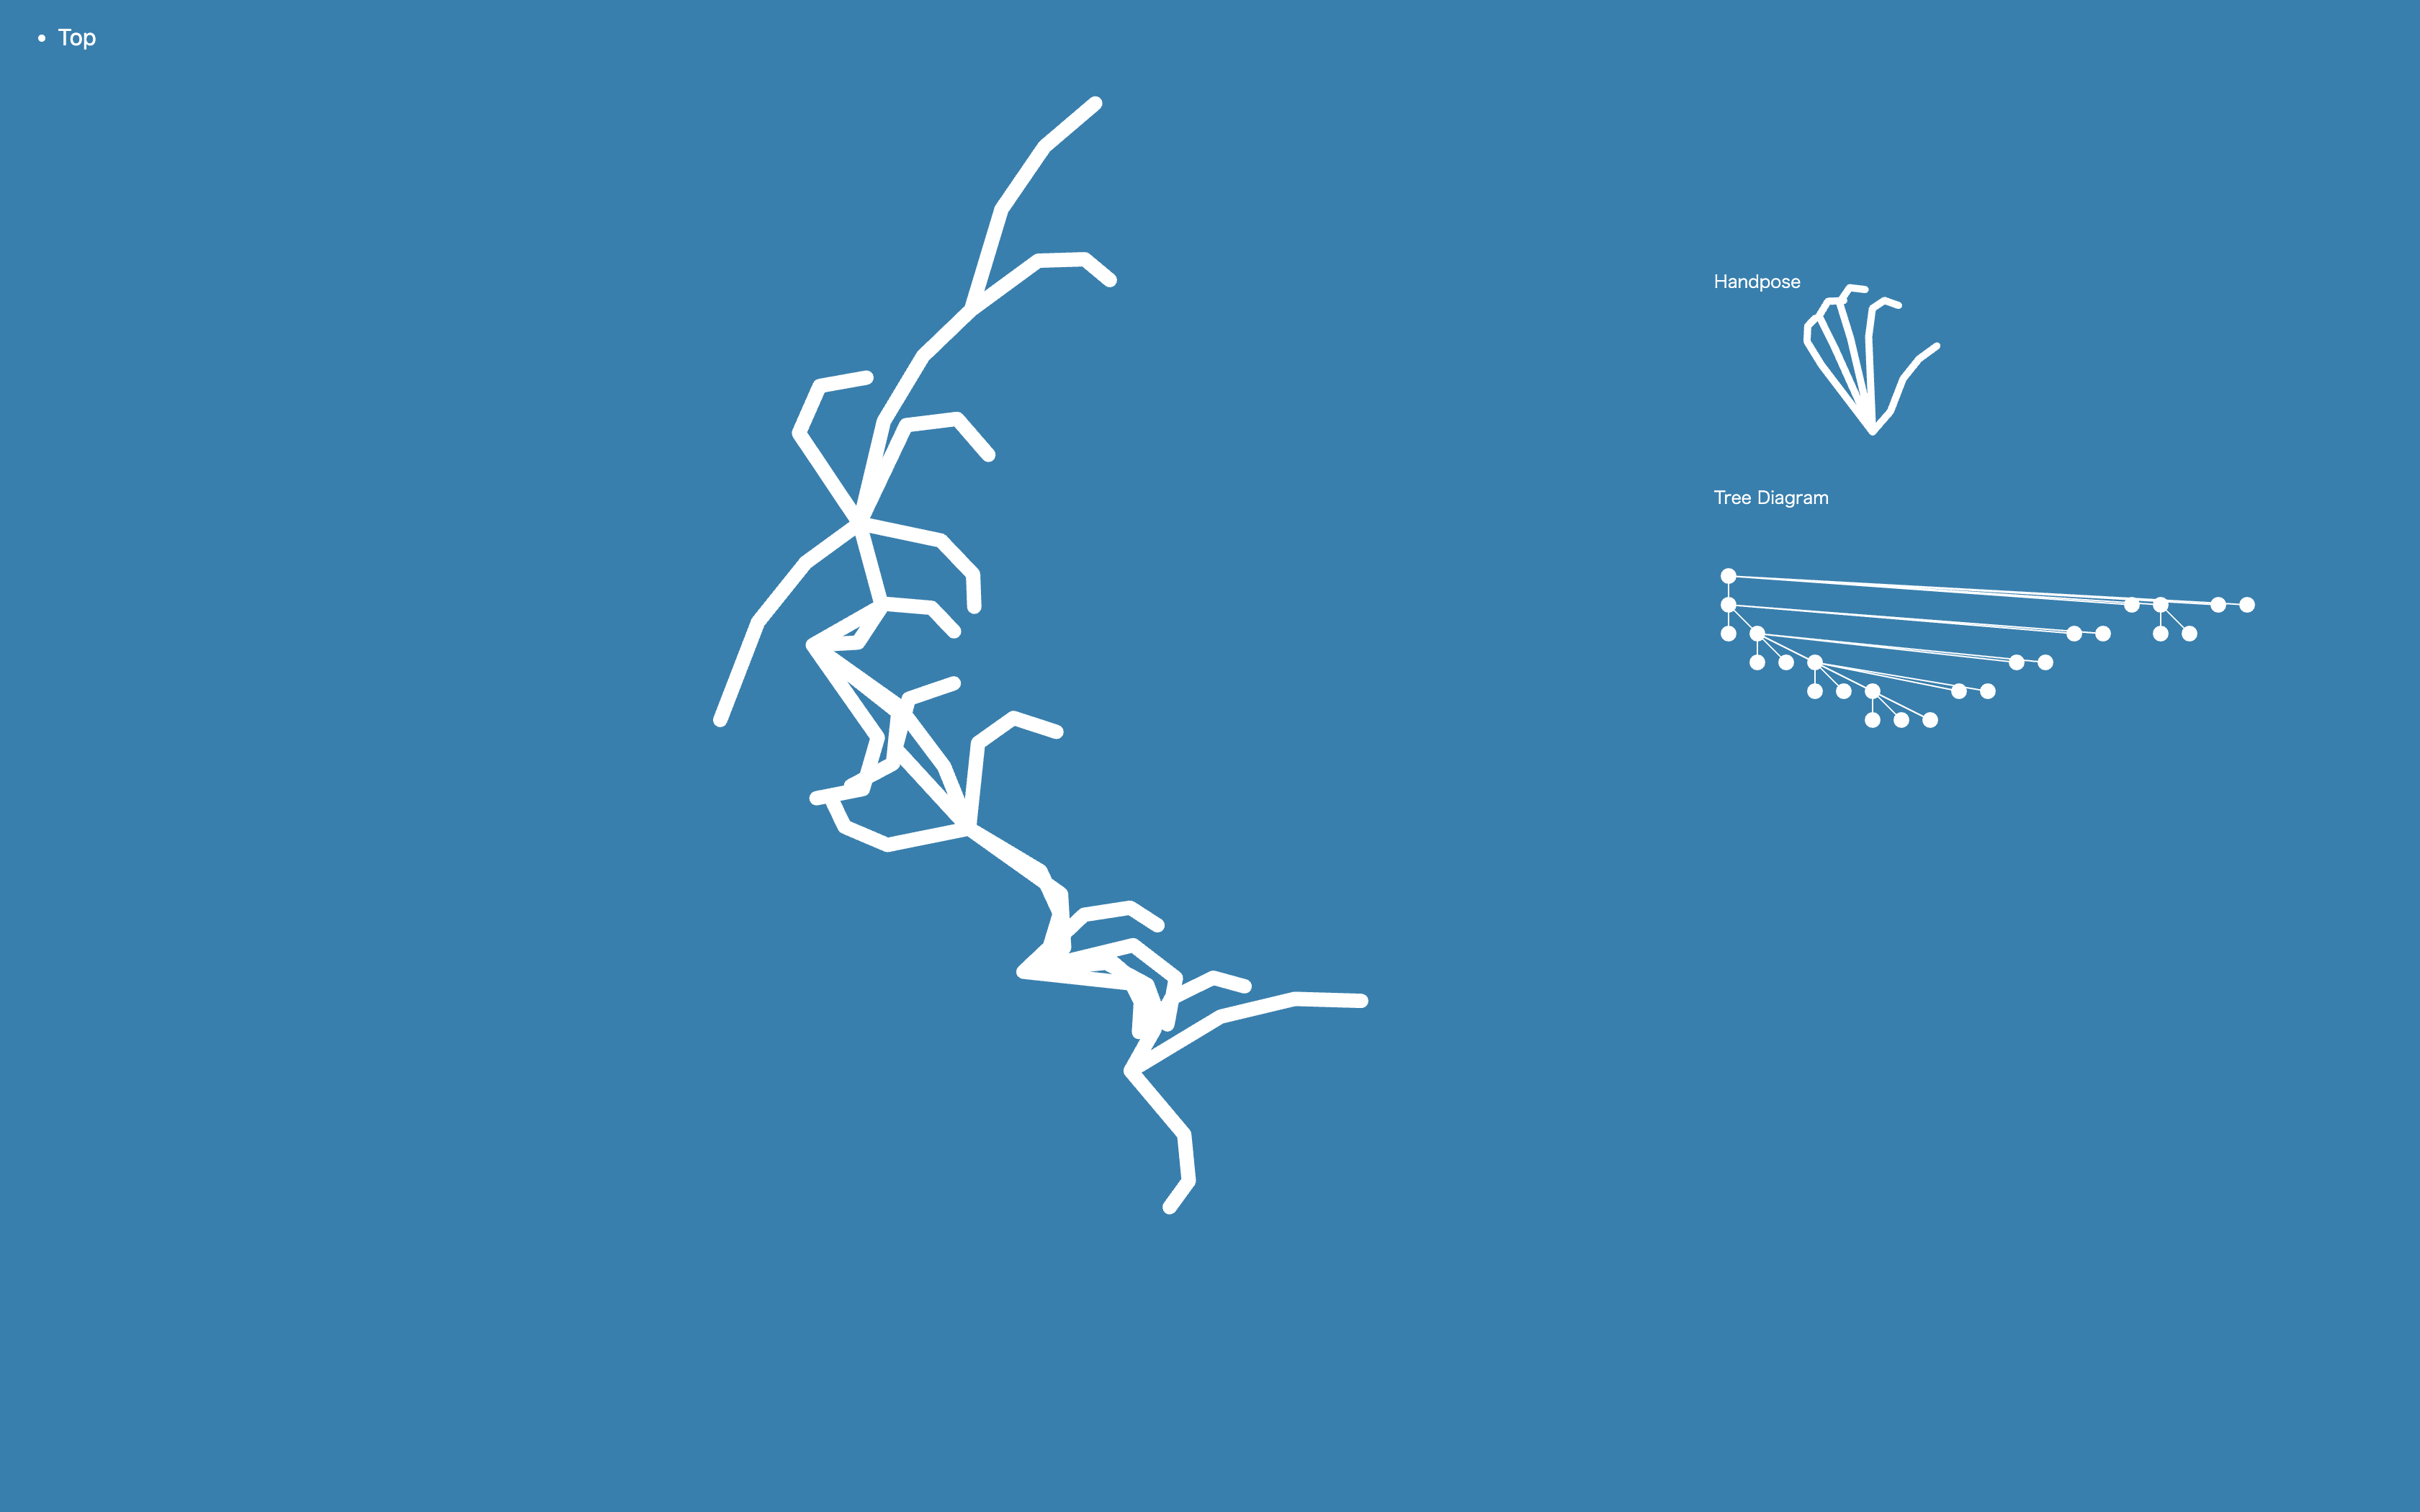
\includegraphics[keepaspectratio, width=7cm]{img/networked_finger.png}
    \caption{Networked Finger}
    \label{fig:networked_finger}
  \end{minipage}
  \begin{minipage}[b]{0.5\linewidth}
    \centering
    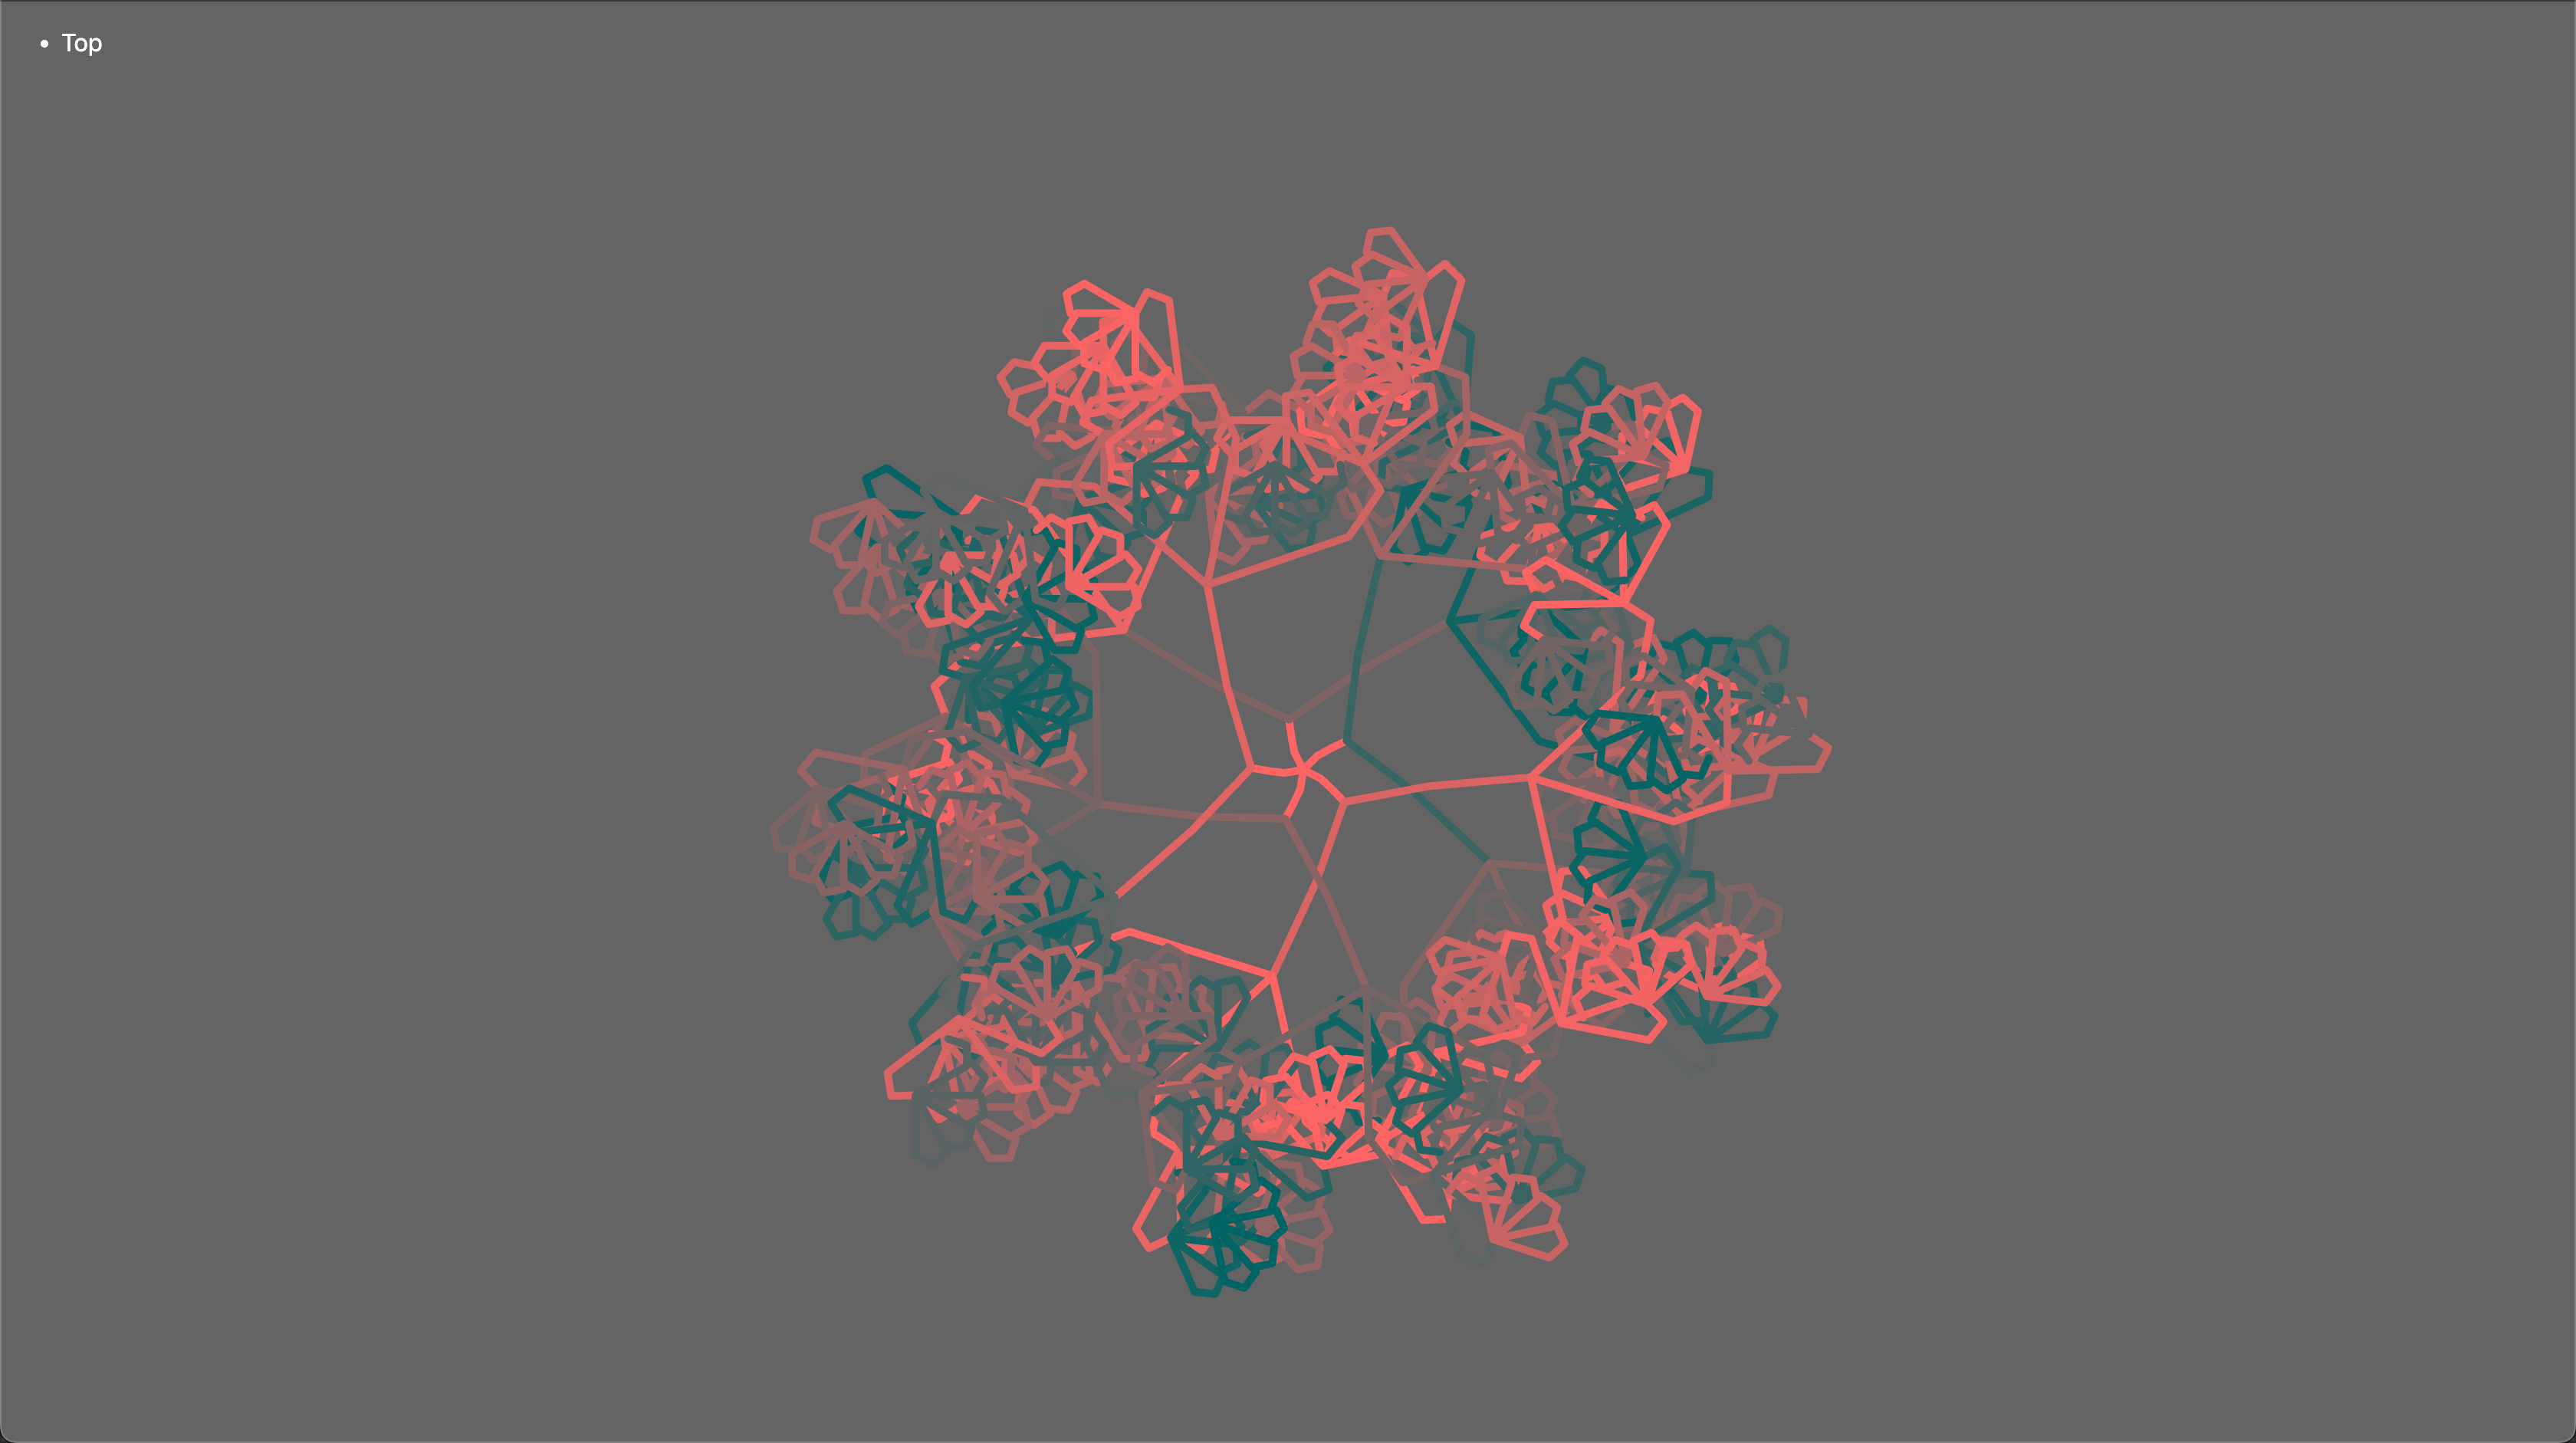
\includegraphics[keepaspectratio, width=7cm]{img/fractel_finger.png}
    \caption{Fractal Finger}
    \label{fig:fractal_finger}
  \end{minipage}
\end{figure}

\subsection{時間操作}
現在の自分の動きだけを表示するのではなく、過去の動きも表示するプロトタイプにも取り組んだ。図\ref{fig:prototype_delay}に示すプロトタイプでは、5本の指の動きが等間隔に並べられているが、それぞれの指は、鉛直上向きの角度に現在の指の動き、そこから時計回りに、順次過去の指の動きが並べられている\footnote{\url{https://interaction005-moe5dbh11-k1105.vercel.app/}}。このプロトタイプでは、指先を小さく動かすと、その動きが時計回りに伝播していくような動きが起こる。これは例えばゼリー状の物体を触れた時のような、物体の衝撃が全体へと伝播していくようすにも見立てられる。そのためか、柔らかいオブジェクトに触れているときのような手触りのようなものを感じた。

\begin{figure}[H]
  \centering
  
\includegraphics[width=15cm]{img/past_time.png}
  \caption{過去の動きを用いた例}
  \label{fig:prototype_delay}
\end{figure}

\subsection{ボール操作}
ここまでは手指をいかに変換するかについて探索を行なってきたが、その手指を用いた動きの複雑度に影響する要素としてボール操作について検討した。

こうしたバリエーションを制作し、ボールがないものと並置して「IAMAS openhouse2023」にて展示した際、体験した方の一人から2つを比較して、手指の変換表現だけのものについては「途中から自分が何やってるか忘れてしまって、なんとなく指を動かすとなんとなく画面の描画内容が変わってる、となってしまっている」一方で「ボールの方はそんなことはなかった」とし、その理由として「具体的なタスクがあったほうがずっと続きやすい」といったことを挙げていた。そのため、よりタスクを明確化したバリエーションとして下記のような、マトあてのバリエーションも制作した。

\begin{figure}[H]
  \centering
  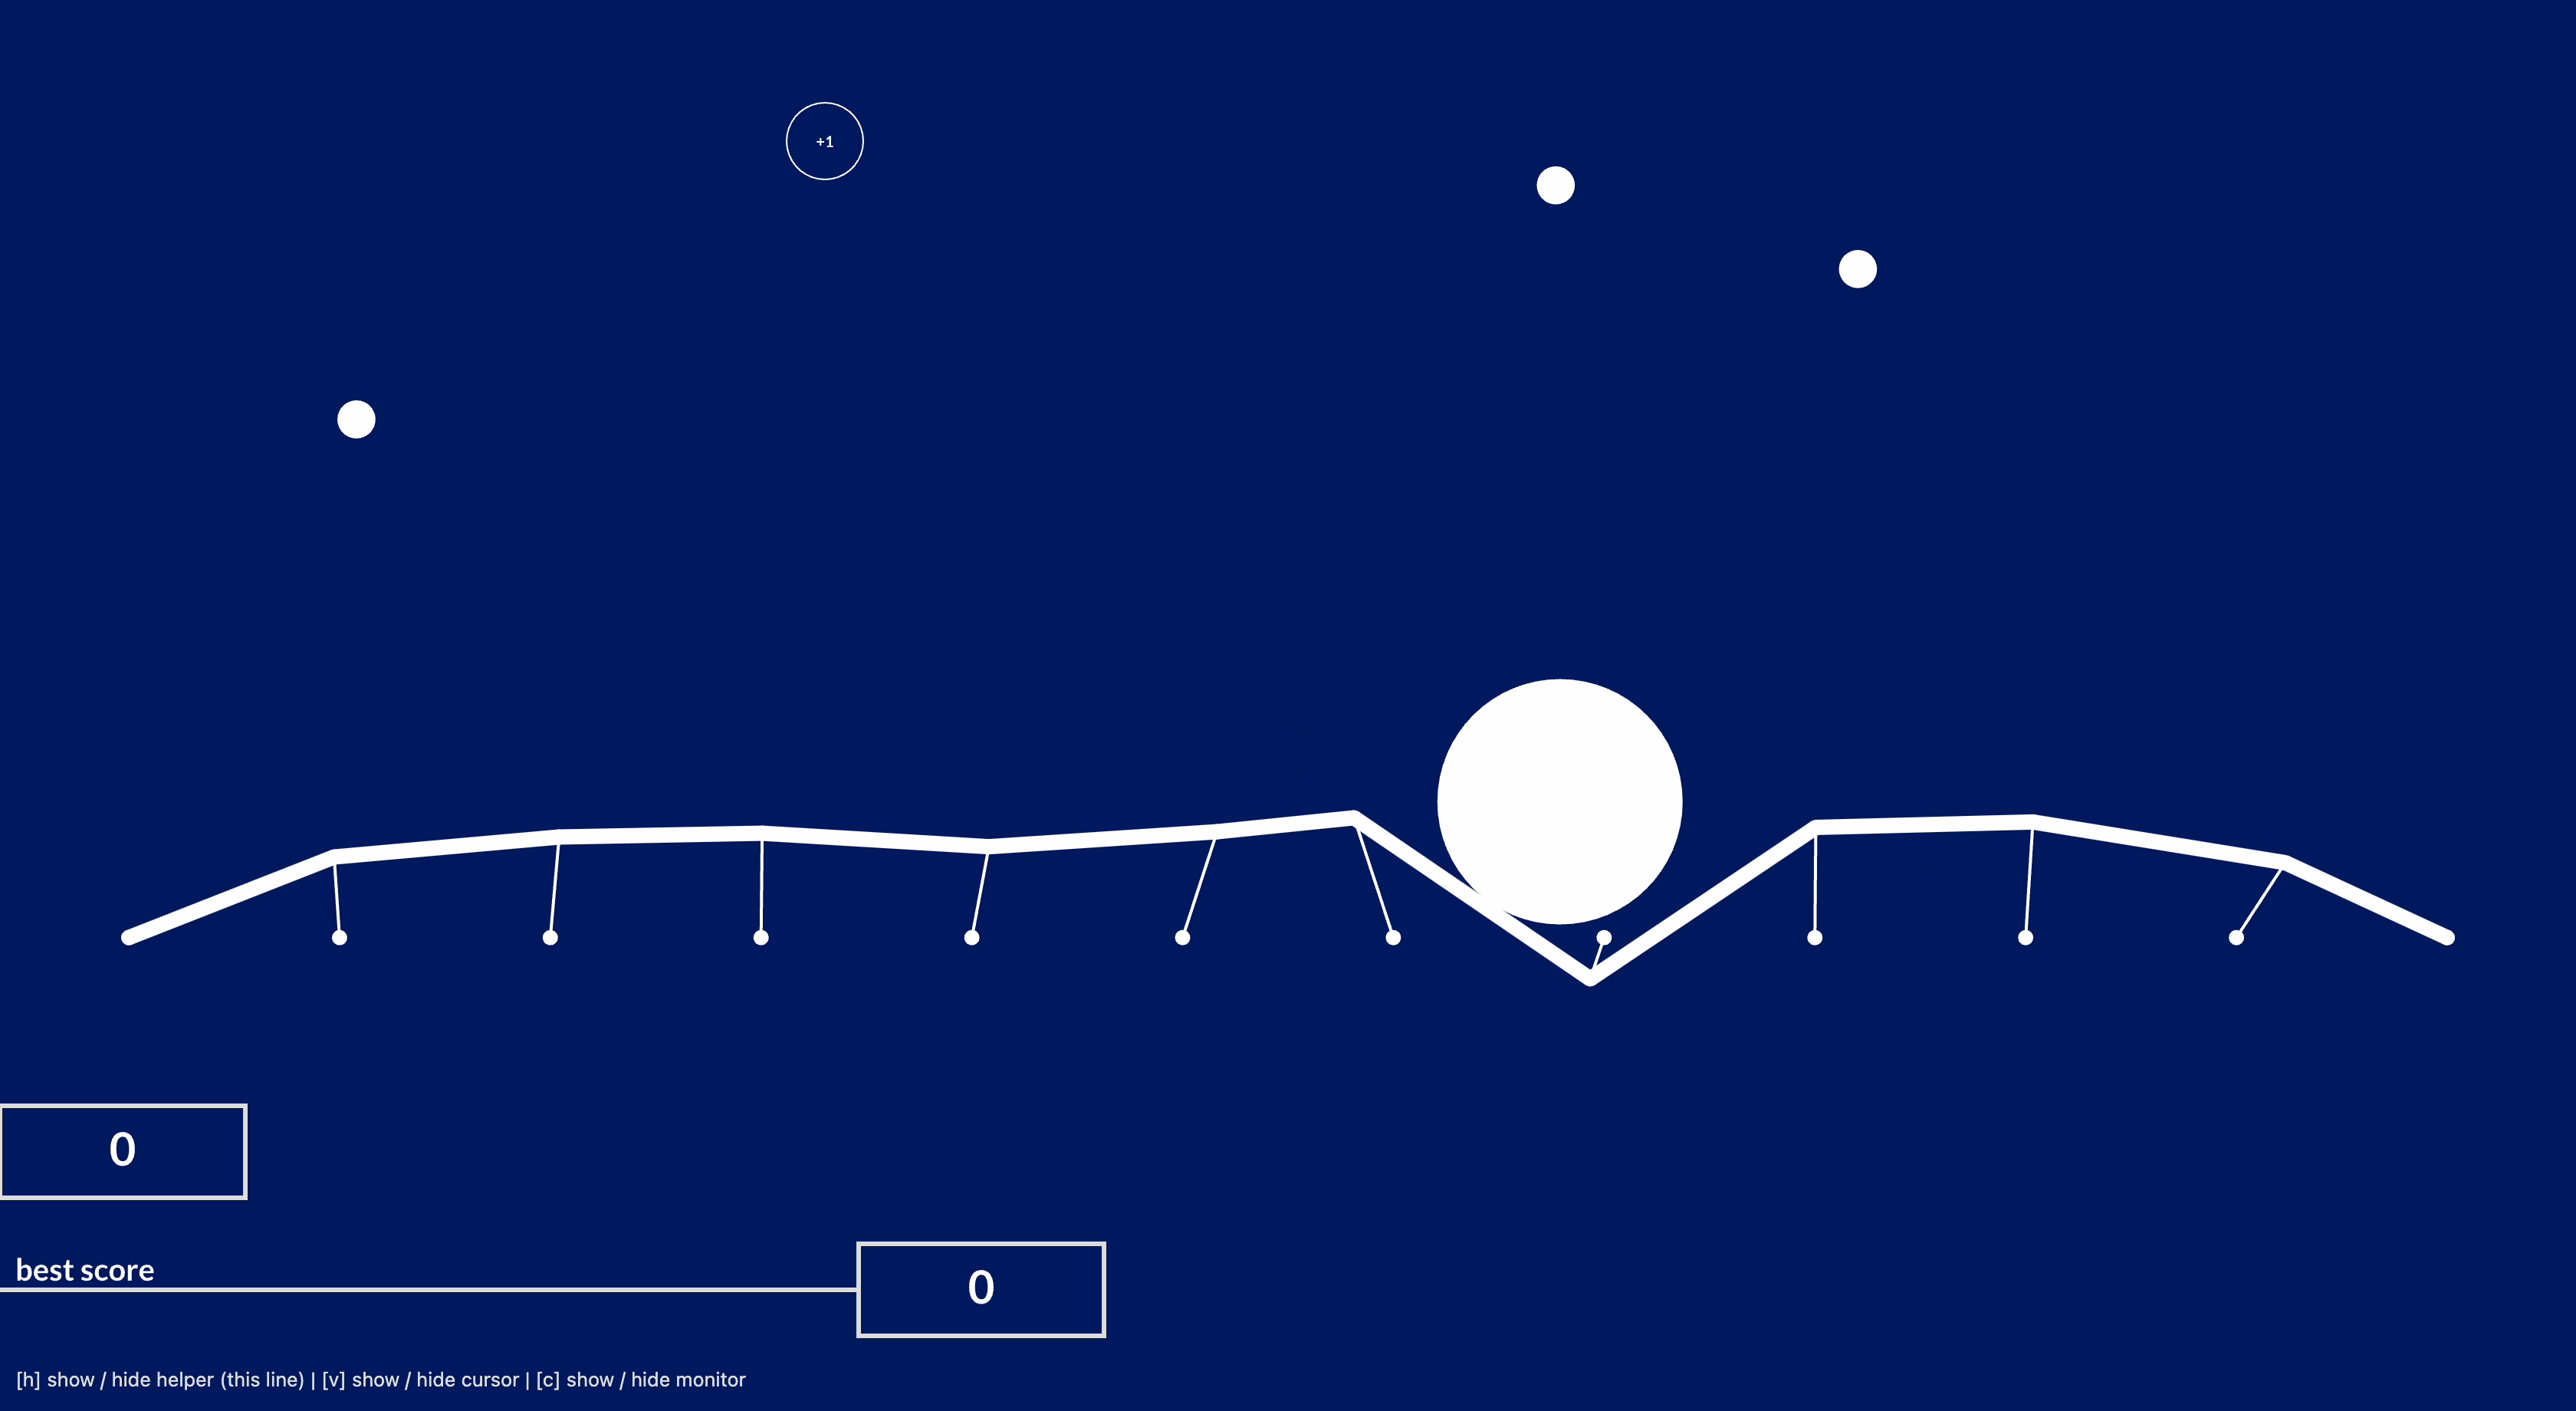
\includegraphics[width=15cm]{img/ball_overview.png}
  \caption{ボール操作の例}
  \label{fig:ball_overview}
\end{figure}

また、過去に制作したバリエーションを拡張する形で、ボール操作のパターンについて検討した\footnote{\url{https://interaction023.vercel.app/}, \url{https://interaction024.vercel.app/}}。

\begin{figure}[htbp]
  \begin{minipage}[b]{0.5\linewidth}
    \centering
    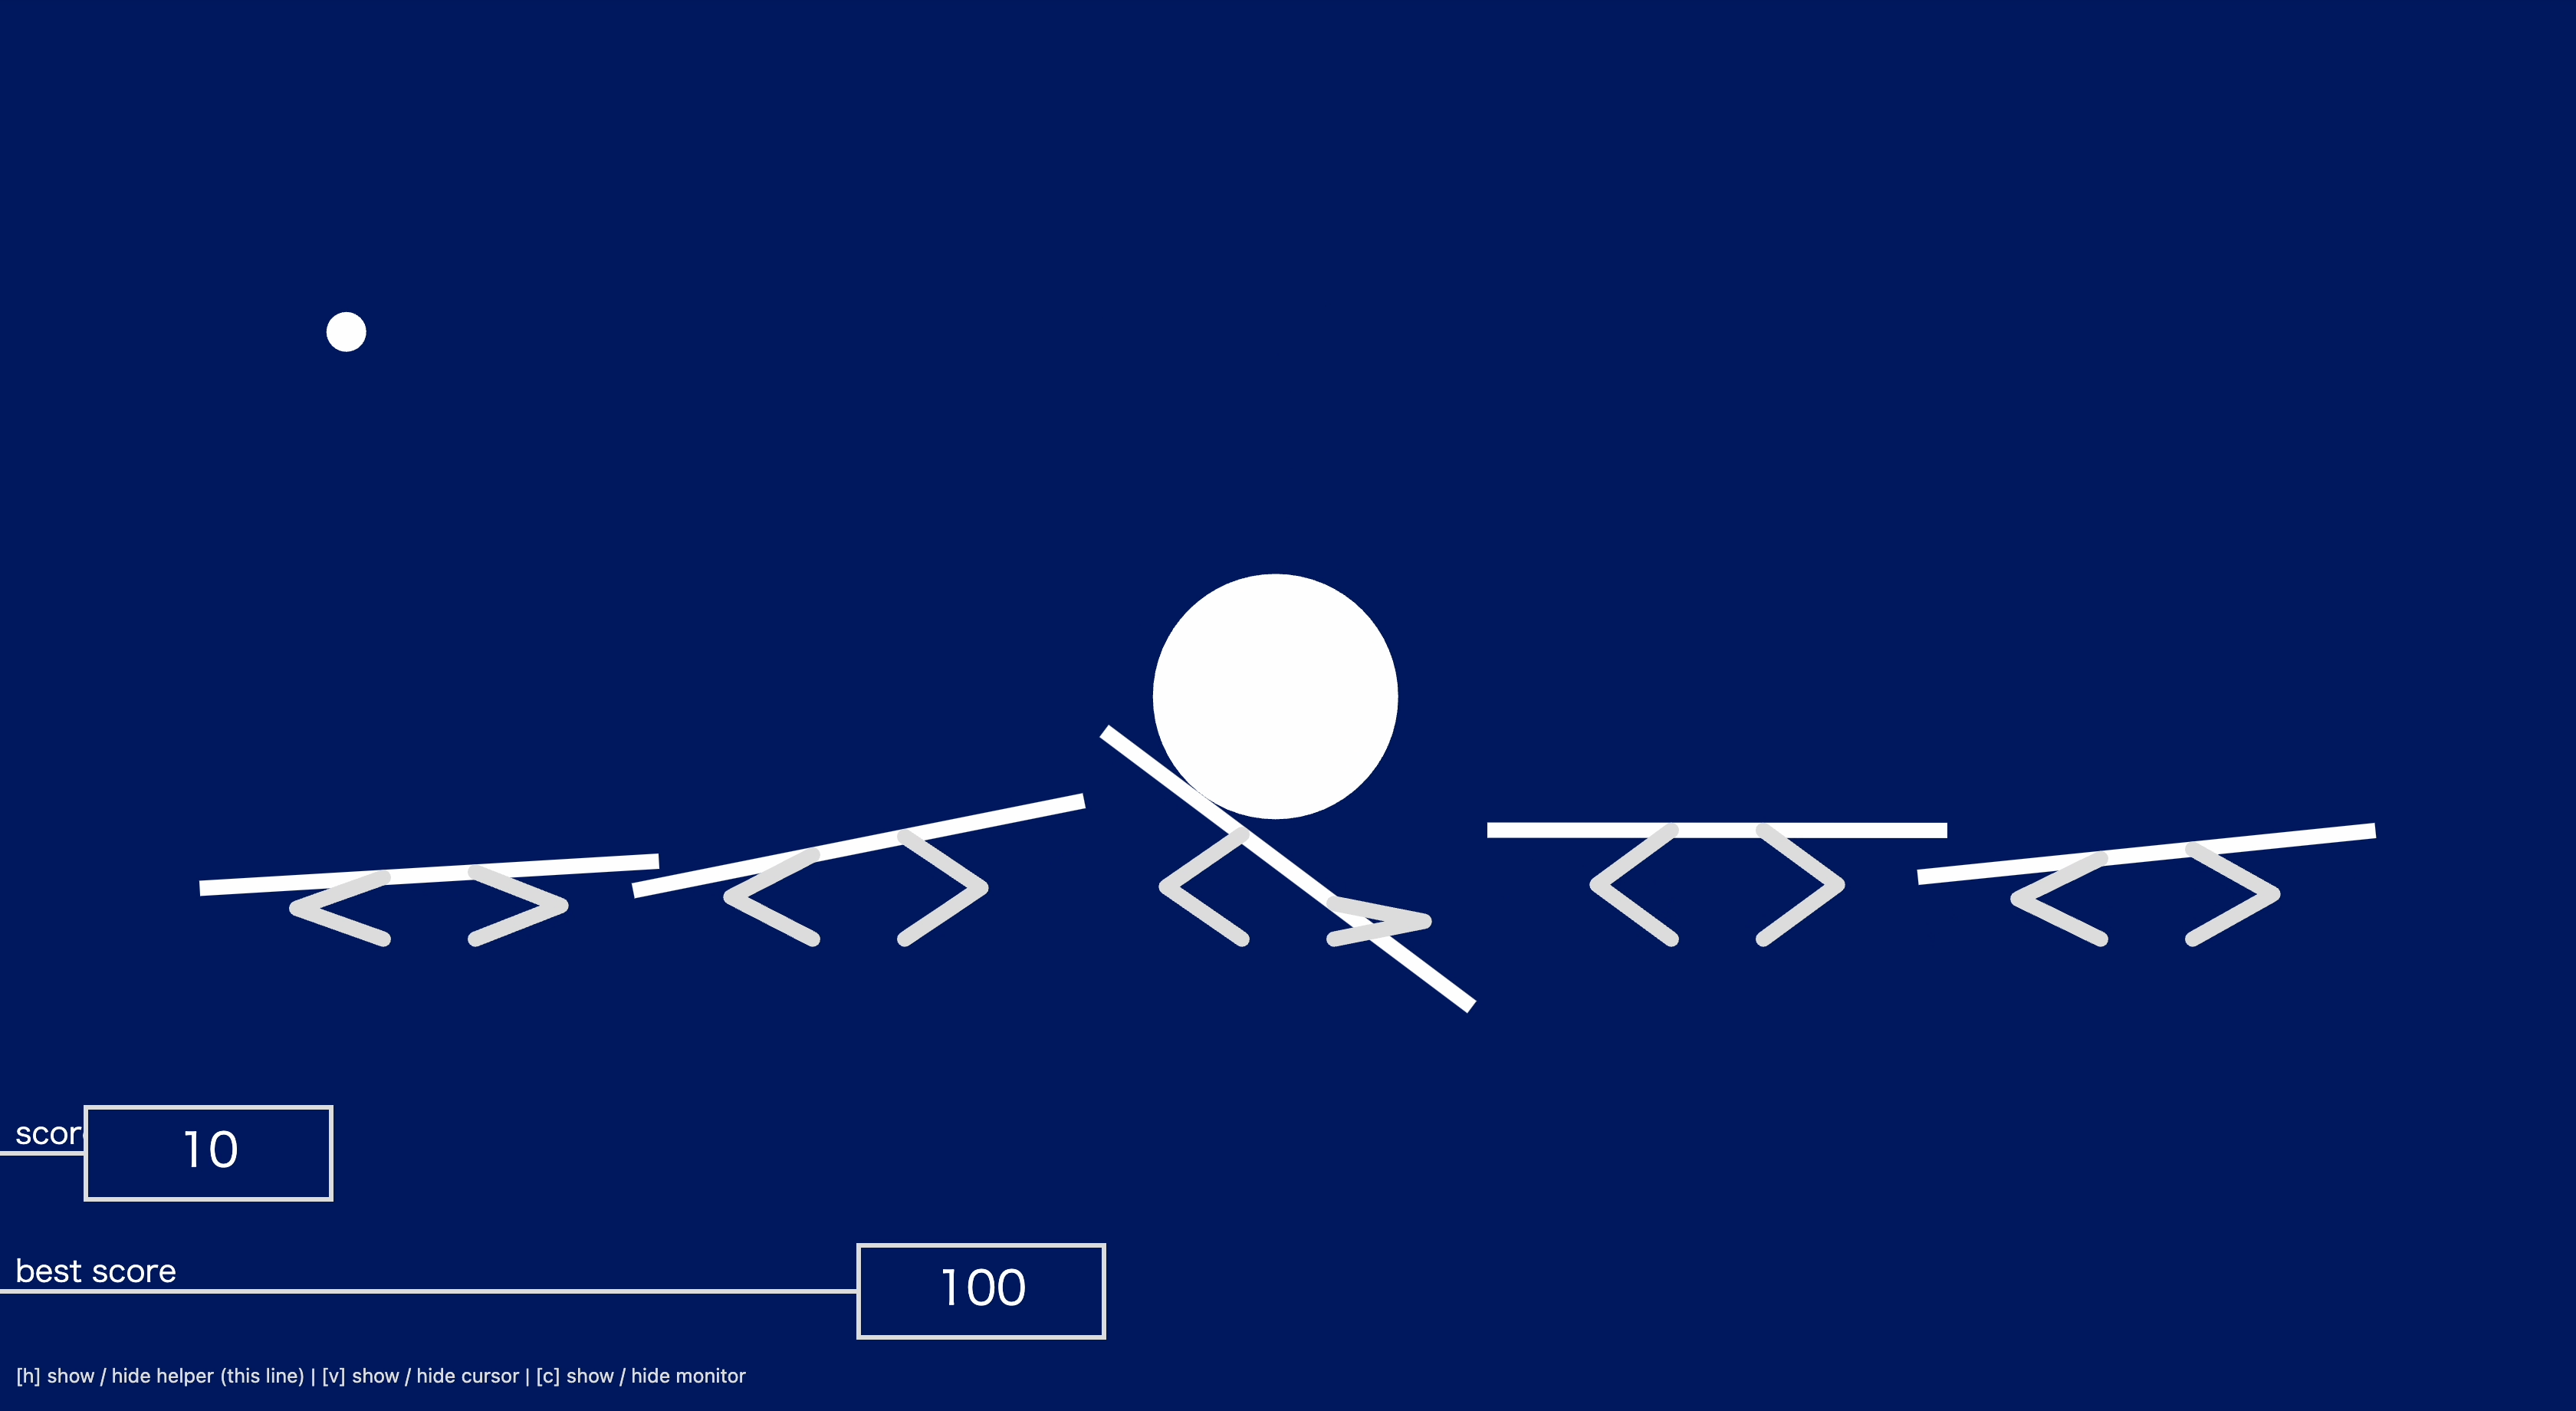
\includegraphics[keepaspectratio, width=7cm]{img/ball_0.png}
    \caption{Networked Finger}
    \label{fig:ball_0}
  \end{minipage}
  \begin{minipage}[b]{0.5\linewidth}
    \centering
    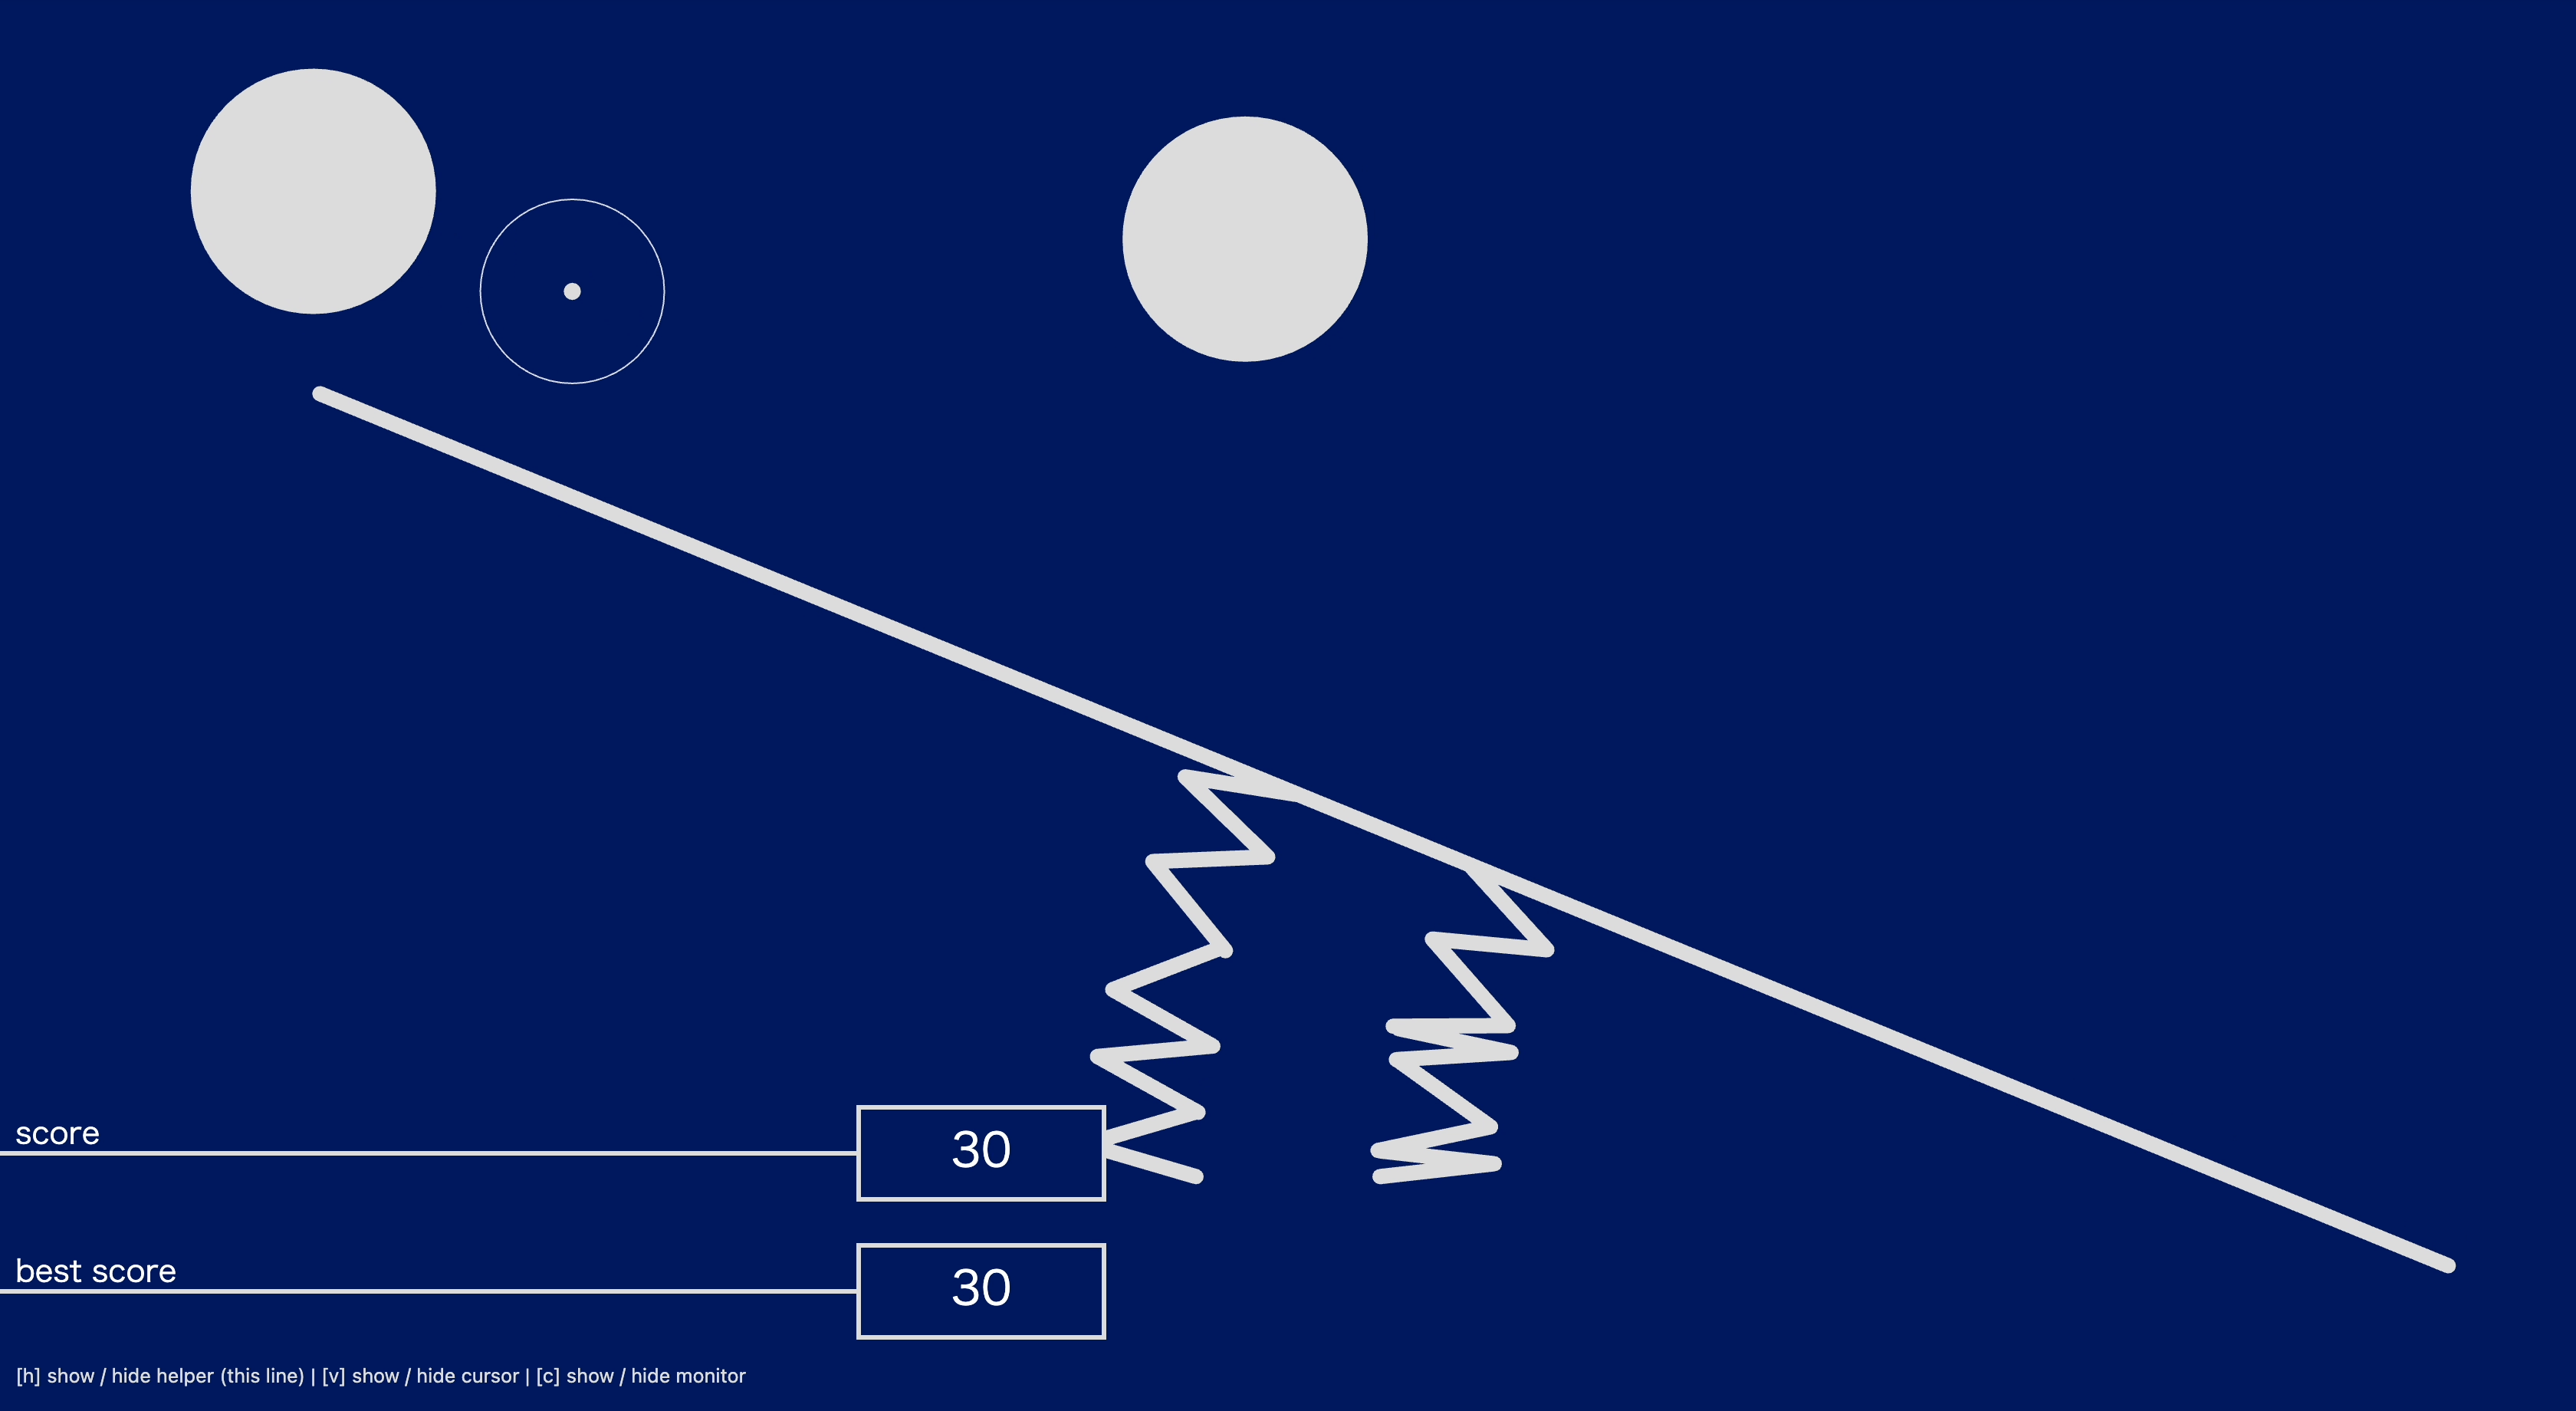
\includegraphics[keepaspectratio, width=7cm]{img/ball_1.png}
    \caption{Fractal Finger}
    \label{fig:ball_1}
  \end{minipage}
\end{figure}

\section{振り返り}
形状については、指を単位としない場合についても検討したが、指は一本一本独立して動かすことができる性質上、指が一つの単位となっている変換に注意を向けやすいのではないかと考えた。その中でも、円形、くの字、ひょうたん型などの変換を試みたが、動きに対して注意が向けられたのは「くの字」の形状であると感じられた。この理由について、身体動作である指の折り曲げとの対応から考察する。

身体動作として指の折り曲げが画面の中で、円の半径へと対応している場合とくの字のような折り曲げ動作に反応している場合とを比べたとき、後者は実際には指先と指の付け根の距離しか評価していないにも関わらず、制御点が3つあるように感じられる。そう捉えると、円の半径が変化していくことよりも対応関係が厳密であり、それを動かすことによって得られる心地よさは、Felsの「Control」による心地よさであると捉えられる。その一方で、円の半径に関節の動きをマッピングさせるような表現については、縮んだり、膨らんだりする動きには共感しづらい。微細な運動が増幅されることに気持ちよさを感じるが、これは身体動作との連動によってもたらされる気持ちよさではなく、動作に対するフィードバックに対する気持ちよさ、すなわちFelsのいう「Response」によるところが強い。

マッピングに関しては、1つの指の動きが規則的に配置される場合について、グラフィックの複雑度が上がっているにも関わらず、感覚としてはより単純な動きであると感じた。これについては、グラフィックデザイナーの女性が体験した際「構造としては緻密であるのに、動きは単純であるように感じる」と意見したことにも重なる。その理由として彼女は、「対称性が前面に出ているため、シンボルとしての印象を強く感じてしまう」「意識していないところも同時に動いている感覚があるため、自分の動きだと思えない」からではないかと推測した。一方で、不規則的に配置される図\ref{fig:networked_finger}のような形状の場合は、1つの動きが複数箇所に複製されているが、指の数が増えると複雑度も比例して上がっているように感じる。これは一つの動きが波及する箇所が多く、動きの予想がつきづらいためではないかと考える。

時間操作の例として示した図\ref{fig:prototype_delay}の例については、数ミリ秒前の動きが隣接する形に現れ、全体として2秒程の期間の全ての動きが表示されることになる。そのため、2秒間のあいだに動きの変化があれば、身体を動かしていても止まっていても画面に変化が現れることが、直感に反した動きとなることに注意が向く。

ボール操作に関しては、身体動作を通して直接的に動かすことのできる対象ではないものが現れたことによって、体験の中に「もどかしさ」が生じたと考える。特に、マトのあるときに、その度合いが強まった。これは、明確かつ簡単に達成することのできない目標設定がされることからではないかと考える。また、マトあての利点として、「一体化」の度合いを「いかに器用にマトに当てることができたか」という観点から、客観的にも、主観的にも確かめることができると考えた。

しかしその一方で、ボールの出現によって手指だけを動かして感覚を確かめていたときとは、全く異質の体験であると感じた。手指の変換のみが行われていた時には、指一本一本の動きや、それによって構成される全体的な動きに注目していたが、ボールが出現したことによってボールと手の関係性にのみ、注目するようになったと考える。

\section{選定と作品構成}
ここまで説明したプロトタイピングと振り返りを踏まえて、最終的な作品構成へ繋がる評価軸や、採用された構成について説明する。
\subsection{動かしている感覚が強い表現}
1つ目の観点として、手指の微細かつ複雑な動きをもって、緻密な制御をしているという感覚が引き出される表現へと絞り込んでいくことにした。そのため、1つの動きを複製して円形に配置したり、フラクタル的に配置するパターンは採用しなかった。また、形状についてのバリエーションでの振り返りを通して、関節の動きが身体動作との関連について想起しやすい変換であると考え、それ以外の展開を採用しなかった。

\subsection{注意の対象による作品の分割}
ボール操作に関するバリエーションを制作した際の気づきから、ボール操作は「もどかしさ」を経験するほどの比較的強い注意を喚起する一方で、ボールがなかった場合と比べると、注意の向く対象が、手指の運動ではなく、ボールと手指の関係性に注意が生じることがわかった。そこで、最終的な作品としてはその2つを分けて構成した。そして、手指の形状が変化することを起点に注意が生じる作品と、ボールと手指との関係性に注意が生じる作品というように、何に注意が生じるかという観点に着目して2つの体験を整理した。

また、ボールの現れる作品においては、プロトタイピングの過程で表示していた「スコア」を設けなかった。理由として、スコアが存在することで「マトに当てる」という目的意識を強く与えてしまうことが挙げられる。強固な目的意識の設計は、より多くの人を同一の目的に向かわせ、一定の体験が期待できる一方で、その目的以外の興味や注意が生じる余地を排斥してしまうと考えた。

\subsection{モーフィングの追加}
過去に展示していたバージョンではモーフィングを示さず、手指が認識されたとたんに全く違う手指が提示される作品形態であった。しかし、この形態で展示した場合、画面の中の手指と自身の関係性について意図しない受け取られ方をすることに気づいた。つまり、全く異なる生命体のようなものを、操り人形のように自分の手指の指令によって動かす、といったような関係性として認識されることがある。また、全く見慣れない形なので「手指を細かく動かせる」といった、作品がもつ可能性に気づけないことがある。そこで、形状の変化を確認できるモーフィングを実装した。そうすることで、白い点が関節を表していること、そして手指の運動を細かくトラッキングしていることを事前に伝え、それが形を変えた姿として画面の前に提示されていることがわかるようになる。

\section{展示形態の設計}
展示形態について、時系列順に過去2つのバージョンについて説明し、その流れから最終的な展示形態の根拠を示す。

\textbf{初期:カメラを画面前に配置した状態}\\
最初期は、体験装置について下図\ref{fig:kyotai_ver0}のように、モデルトラッキングを行っているカメラを直接画面の前に配置していた。
\begin{figure}[H]
  \centering
  \includegraphics[width=12cm]{img/kyotai_ver0.jpg}
  \caption{初期:カメラを画面前に配置した状態}
  \label{fig:kyotai_ver0}
\end{figure}

プロトタイピングの段階でもあったため最低限の構成としていたが、この構成には次のような問題があった。
\begin{quote}
  \begin{itemize}
    \item カメラのトラッキング精度が環境光の影響を受けて変動してしまう
    \item 体験者ではない周囲の人の手指を間違ってトラッキングしてしまう
    \item 手指の形がそのまま出力されるわけではないので、トラッキングの範囲がわからず、腕を大きく振ったり、手指がトラッキングできない範囲で動かしてしまう
  \end{itemize}
\end{quote}

このため、制作者が指示をすることなく自由に体験してもらうことを意図していた展示であっても、体験方法がわからなかったり、後方で見守る人の手を誤ってトラッキングしてしまうといった問題が起き、有効なフィードバックを得ることができなかった。

\textbf{中期:専用筐体を用いて手首を固定した状態}\\
こうした課題を踏まえて、次に専用筐体を制作し、穴に手を入れる形式について試した(図\ref{fig:kyotai_ver1})。

\begin{figure}[H]
  \centering
  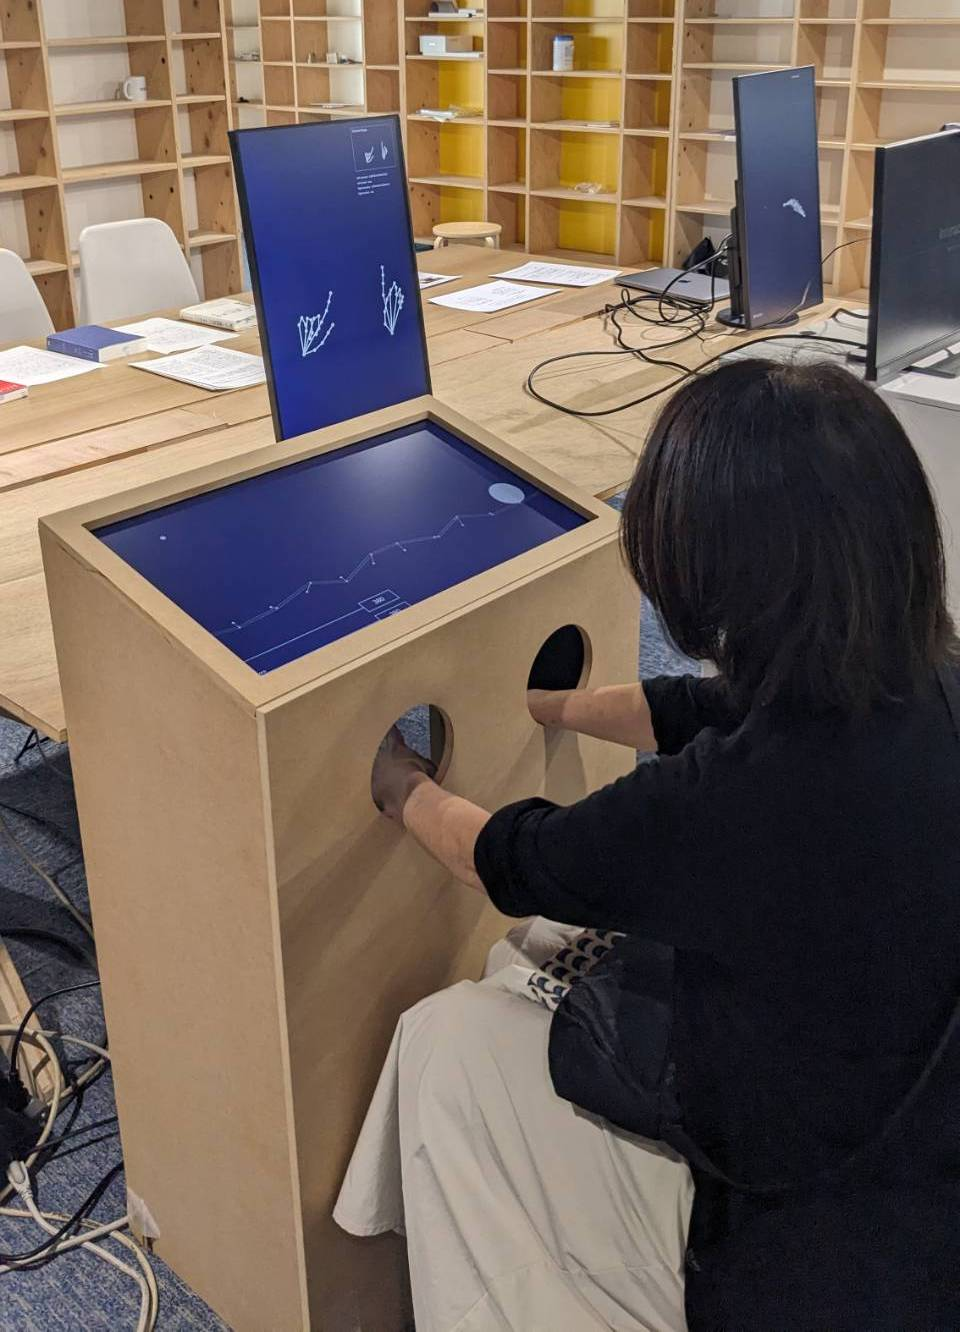
\includegraphics[width=8cm]{img/kyotai_ver1.jpg}
  \caption{中期:専用筐体を使用してカメラを隠蔽した状態}
  \label{fig:kyotai_ver1}
\end{figure}

この形式では、カメラの画角に映り込むのは筐体の内部と体験者の手のみであるため、環境光の影響や周囲の人の影響を受けずに体験できるようになった。また、穴によって手首の位置が固定されるため、腕を大きく振ることが構造上不可能となり、比較的身体動作の幅が抑えられた。

ただし、この形式は単に上記の問題を解決したというだけではなく、指先の動きが見えなくなったこと、画面に対する指先の位置関係についてを変更するものであった。

画面に対する手指の位置関係については、本作品では手指の形状が、もとの形とは全く関係のない構造へと変化するため、作品体験には大きな影響はないと判断した。手指の動きが見えなくなったことについては、画面の中の手指は体験時、自身の身体に代わる存在であるから、同時に視認できない今の形態の方がむしろ、より適した構成であると判断した。

しかしその一方で、手首の動きを固定してしまったことは、身体の動きを過剰に限定してしまう結果となった。身体の動きを限定してしまうと、何か特定の動作を求められているような説明的な構成になってしまう。そのため筐体としては、より簡素な構成が好ましいと判断した。


\textbf{作品展示:専用筐体を用いて手首を固定せず指先を自由にした状態}\\
そこで最終的には、図\ref{fig:kyotai_ver2}のような、トラッキングの範囲を暗示しながら、手首を固定しない方式に変更した。また、トラッキングに用いるカメラを、視野角150°の広角カメラ(Sanwa Supply CMS-V43BK-3)に変更し、大きく手指を動かしてもトラッキングの外れることの少ないものへと変更した。

\begin{figure}[H]
  \centering
  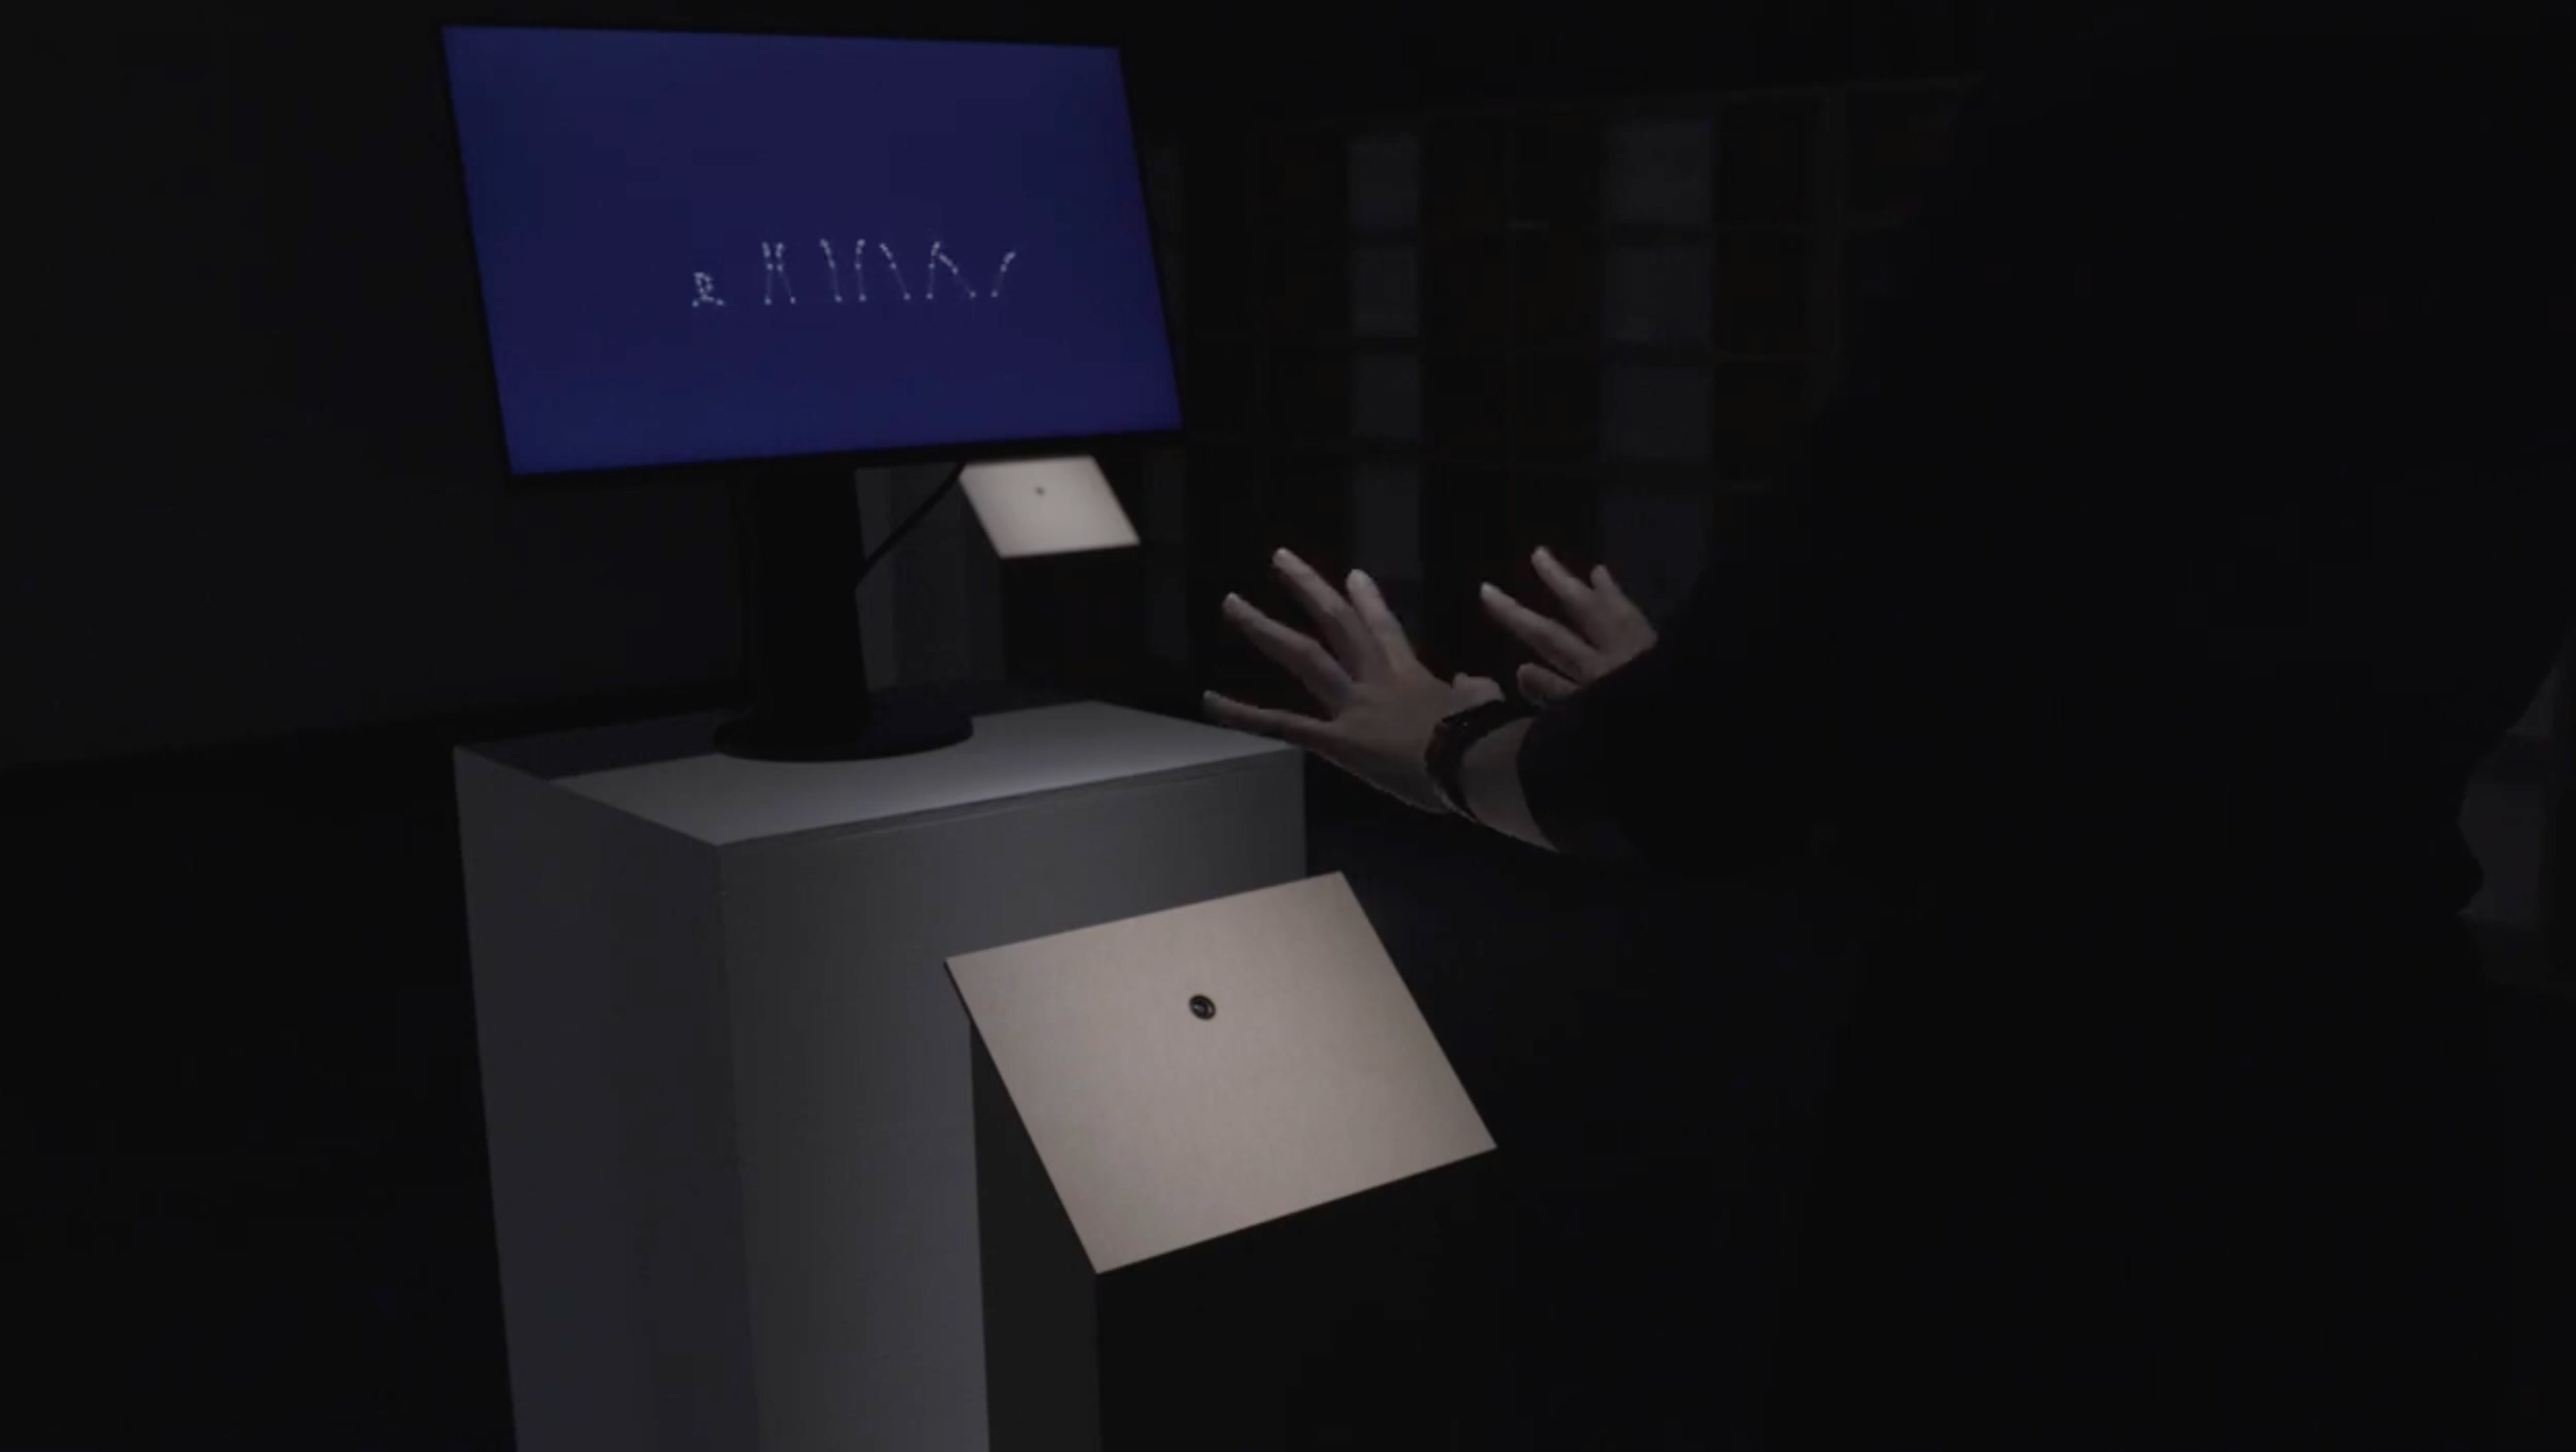
\includegraphics[width=12cm]{img/kyotai_ver2.png}
  \caption{作品展示の際の筐体}
  \label{fig:kyotai_ver2}
\end{figure}

筐体の高さは腰ほどの高さ(850mm)とすることで、キーボードのブラインドタッチのように、画面を見ながら手を同時に見ることが難しい構成とした。

カメラは、鉛直上向ではなく斜めを向いているので、筐体の前に立つと体験者の身体と手指の位置が重なり、トラッキングしやすい状況ができる。

また、ライティングの調整によってトラッキングの精度を高めた。
最終的な展示形態では、スポットライトを当てることで筐体周りを明るくすると同時に照り返しで手元の採光をし、周囲の照明を落とすことで明暗差を作ることで、手指の姿勢を認識しやすくなる。

\begin{figure}[H]
  \centering
  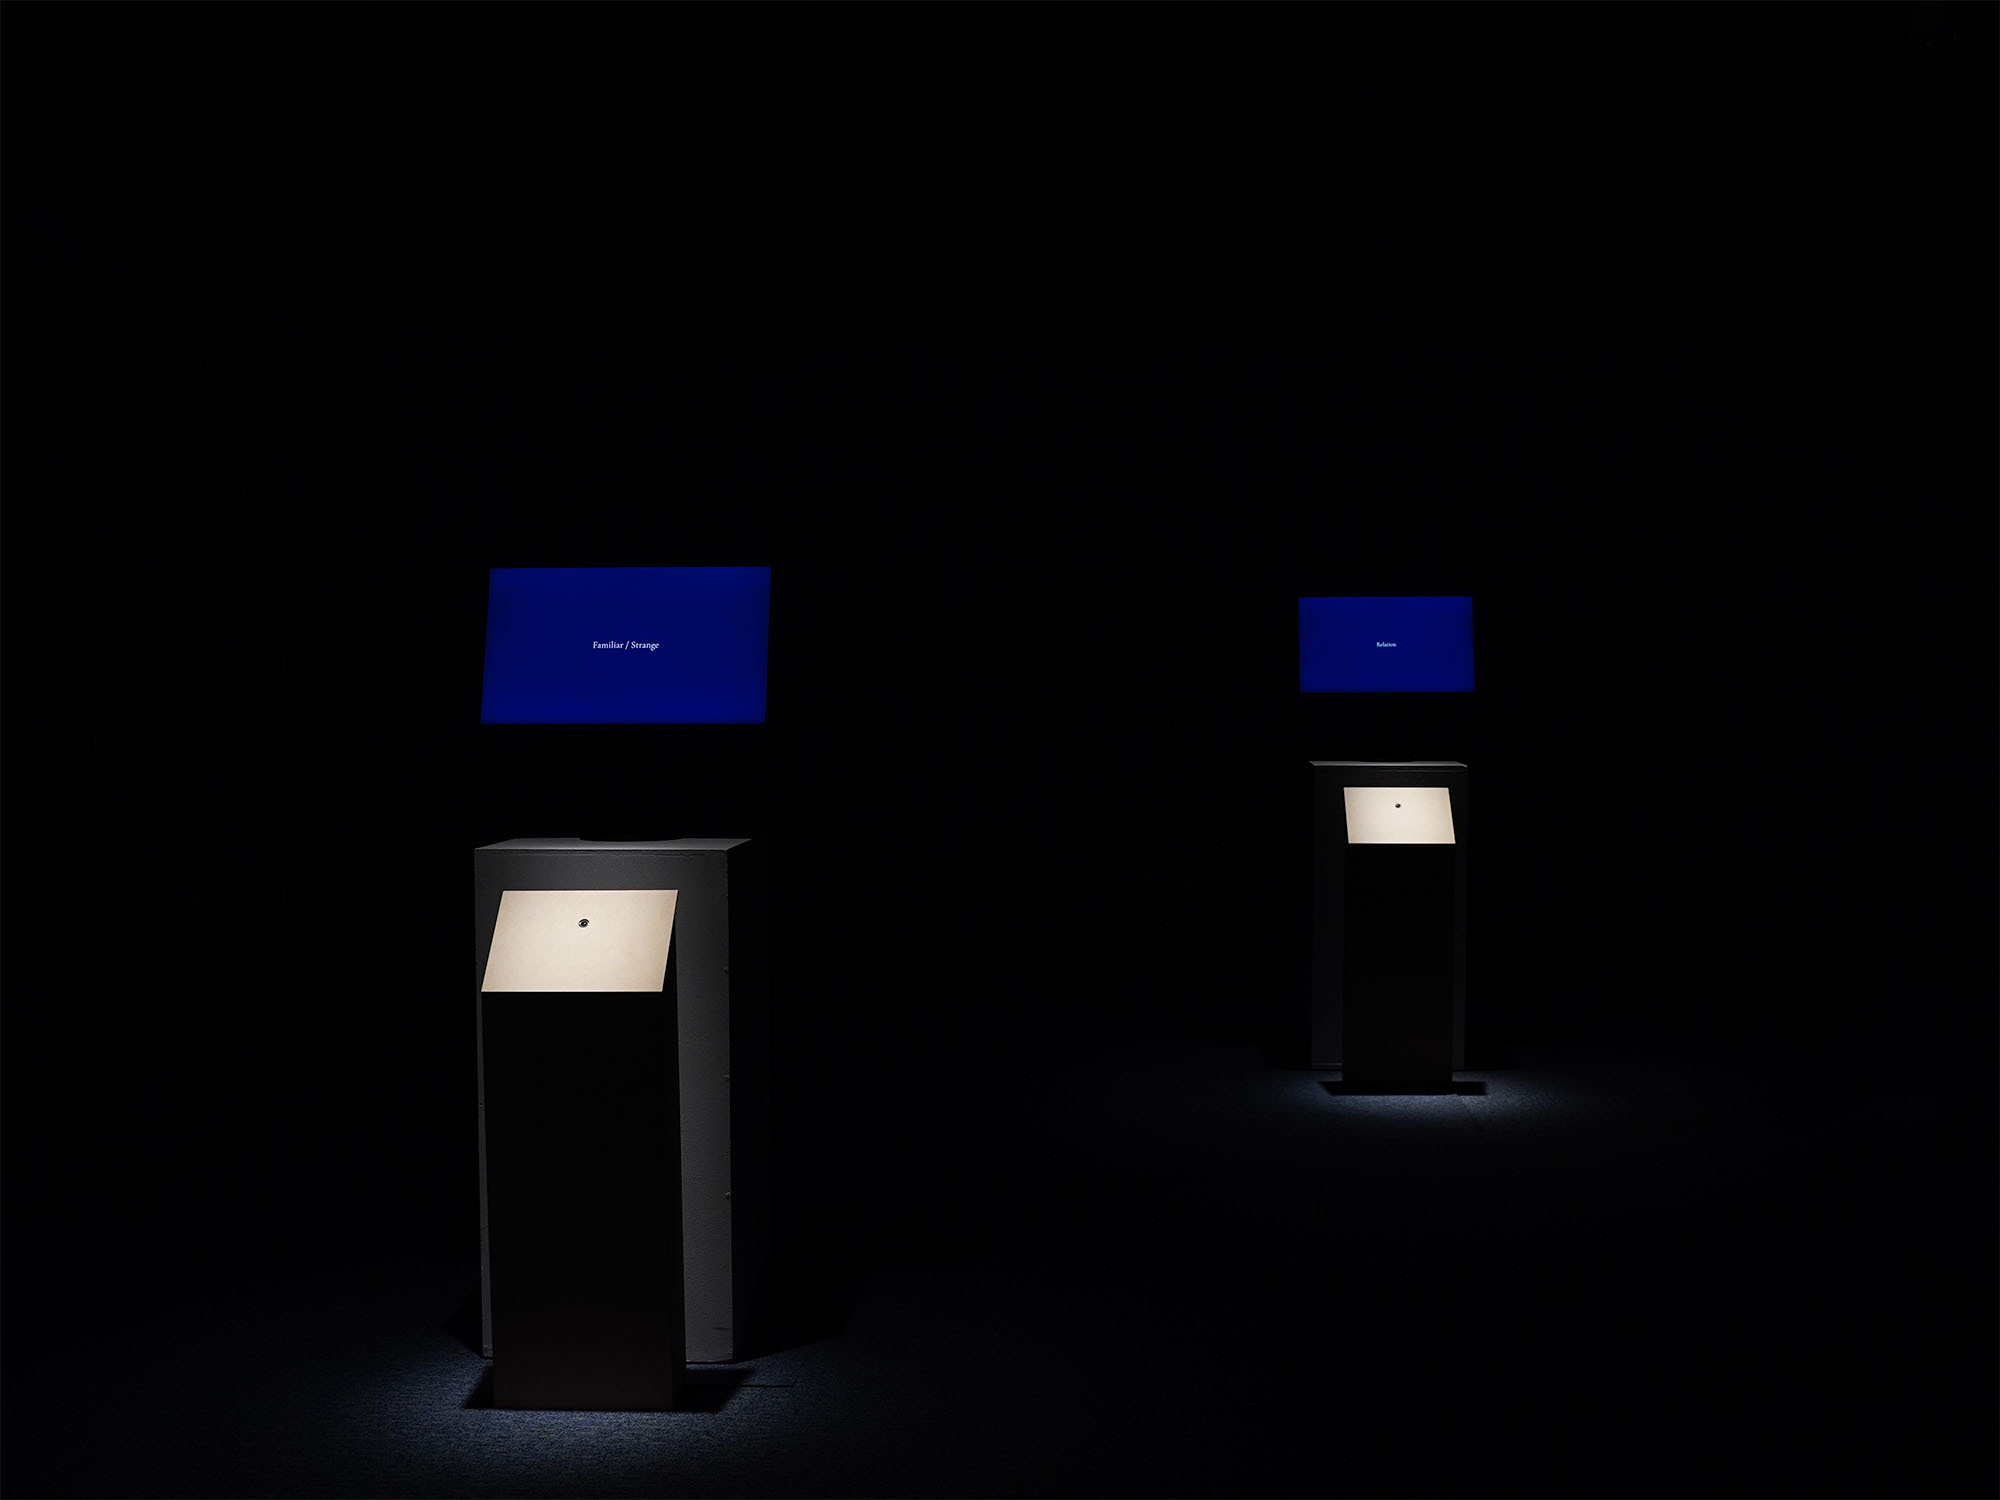
\includegraphics[width=12cm]{img/lighting.jpg}
  \caption{作品展示の際のライティング}
  \label{fig:lighting}
\end{figure}
